\chapter{Species and forms\label{chap:species}}
Pokémon are partitioned into species.
Each species is identified by its own Pokédex number.
We will see that this number is the only thing guaranteed to be shared among all the population of a species.

\section{Forms\label{sec:forms}}
Some species boast multiple forms and genders, all sharing one common Pokédex entry.
Form can be a mere visual distinction, but it is sometimes reflected in stats or even typing.
All Pokémon of a form share Attack (ATK), Defense (DEF), and Stamina (STA) base statistics.
These statistics are always positive integers.

Common forms include \textit{Mega}, a temporary form with greater ATK and DEF (\autoref{sec:mega}),
  \textit{Dynamax} and \textit{Gigantamax}, temporary forms with the ability to use
  powerful attacks (\autoref{sec:dmaxgmax}),
  and \textit{Shiny}, a visually distinctive and rare form (\autoref{sec:shiny}).
Regional variants are also seen: Alolan, Galarian, Hisuian, and Paldean.
Gender differentiation is typically small changes to appearance or call,
 but it affects a few evolutionary paths (\autoref{table:sexevolutions}).
Meowstic and Indeedee have different possible attacks based on their gender,
 Oinkologne has different stats, and Nidoran two entirely different
 species: ``Nidoran♂'' and ``Nidoran♀'' (I have Questions about Nidoran biology).
\begin{table}
\footnotesize
\centering
\begin{tabular}{lll}
Base & Requirements & Result \\
\Midrule
Female Combee	& 50 Combee Candy & Vespiquen\\
Female Salandit & 50 Salandit Candy & Salazzle\\
Female Snorunt & 100 Snorunt Candy + 
\includegraphics[width=1em,height=1em]{images/sinnohstone.png} & Froslass\\
Male Snorunt & 100 Snorunt Candy & Glalie\\
Female Kirlia & 100 Ralts Candy & Gardevoir\\
Male Kirlia & 100 Ralts Candy + 
\includegraphics[width=1em,height=1em]{images/sinnohstone.png} & Gallade\\
Female Burmy & 50 Burmy Candy & Wormadam\\
Male Burmy & 50 Burmy Candy & Mothim\\
\end{tabular}
\caption[Gender-dependent evolutions]{Certain evolution paths depend on gender. Note that male Combees and male Salandits cannot evolve.\label{table:sexevolutions}}
\end{table}

\section{Evolution\label{sec:evolution}}
Under the correct conditions, some species can evolve into others.
We call the set of Pokémon related by evolution operations a genus.
Change of form is not an evolution, since the species and Pokédex number remain the same.
We call a Pokémon that has undergone $N$ evolutions a Stage $N+1$ Pokémon.
No Pokémon of Stage 4 or higher exist.
Evolution (unlike some form changes) is irreversible.
Evolution does not necessarily preserve typing, i.e.\ typing is not always constant within a genus (\autoref{table:heteroevolve})\footnote{It is interesting
  that Sharpedo changes from Water+Dark to Mega Sharpedo's Dark+Water,
  a functionally equivalent typing. When this kind of thing happens,
  I assume it due to conformance with other Pokémon games, but never
  rule out simple fuckups. ALSO, no species lose Dark in an evolution,
  though several gain it. Is Nintendo hinting at the inevitable triumph of
  evil over good, or commenting on the blasphemies central to evolutionary theory?
  Impossible to know, but I'm pretty sure it's one of those things.}.
Evolution infrequently changes the cost group---always in the more expensive direction\footnote{Most
  cost-changing evolutions involve Baby Pokémon.}(\autoref{table:heterocost}).
\input{out/hetero}
Almost all evolutions require Candy of that genus (Zygarde and Gimmighoul are exceptions),
  and some evolutions depend upon some condition (\autoref{table:condevolutions}),
  or walking the Pokémon while your Buddy (\autoref{table:walkevolutions}),
  or a catalyzing item, which is consumed (\autoref{table:itemevolutions}).
Some evolutions can be performed at no Candy cost if the Pokémon was received by trade
 (\autoref{table:tradeevolution}).
Evolution usually improves base stats (though there are many exceptions to this rule),
  and typically makes available new, more powerful attacks.
Evolution revives a Pokémon if it is fainted, and always fully restores HP\@.
\begin{table}
\footnotesize
\centering
\begin{tabular}{lll}
  Base & Requirements & Result \\
  \Midrule
  Magneton & 100 Magnemite candy + active 
\includegraphics[width=1em,height=1em]{images/magneticlure.png} & Magnezone\\
  Nosepass & 50 Nosepass candy + active 
\includegraphics[width=1em,height=1em]{images/magneticlure.png} & Probopass\\
  Charjabug & 100 Grubbin candy + active 
\includegraphics[width=1em,height=1em]{images/magneticlure.png} & Probopass\\
  Sliggoo	& 100 Goomy candy + rain or active 
\includegraphics[width=1em,height=1em]{images/rainylure.png}& Goodra\\
  Bisharp	& 100 Pawniard candy + win 15 
\includegraphics[width=1em,height=1em]{images/dark.png} or 
\includegraphics[width=1em,height=1em]{images/steel.png} raids & Kingambit\\
  Primeape & 100 Mankey candy + defeat 30 
\includegraphics[width=1em,height=1em]{images/psychic.png} or 
\includegraphics[width=1em,height=1em]{images/ghost.png} & Annihilape\\
  Floette	& 100 Flabébé candy + earn 20 hearts & Florges\\
  Charcadet	& 50 Charcadet candy + defeat 30 
\includegraphics[width=1em,height=1em]{images/psychic.png}& Armarouge\\
  Charcadet	& 50 Charcadet candy + defeat 30 
\includegraphics[width=1em,height=1em]{images/ghost.png}& Ceruledge\\
  Poipole & 200 Poipole candy + capture 20 Dragon-type & Naganadel\\
  Hisuian Qwilfish & 50 Qwilfish candy + win 10 raids & Overqwil\\
  Kubfu	& 200 Kubfu candy + win 30 
\includegraphics[width=1em,height=1em]{images/water.png} raids/Max battles & Rapid Strike Urshifu\\
  Kubfu	& 200 Kubfu candy + win 30 
\includegraphics[width=1em,height=1em]{images/dark.png} raids/Max battles & Single Strike Urshifu\\
  Inkay	& 50 Inkay candy + rotating the mobile device & Malamar\\
  Amaura & 50 Amaura candy, and evolve at night & Aurorus\\
  Tyrunt & 50 Tyrunt candy, and evolve during the day & Tyrantrum\\
  Pancham	& 50 Pancham candy + capture 32 
\includegraphics[width=1em,height=1em]{images/dark.png} & Pangoro\\
  Ursaring & 100 Teddiursa candy during full moon & Ursaluna\\
  Galarian Farfetch'd & 50 Farfetch'd candy + 10 Excellent throws & Sirfetch'd \\
  Spritzee & 50 Spritzee candy + use incense & Aromatisse\\
  Swirlix & 50 Swirlix candy + feed 25 treats & Slurpuff\\
  Galarian Yamask & 50 Yamask candy + win 10 raids & Runerigus\\
\end{tabular}
  \caption{Evolutions dependent upon a condition\label{table:condevolutions}}
\end{table}
\begin{table}
\footnotesize
\centering
\begin{tabular}{lll}
  Base & Usual requirement & Result \\
\Midrule
Kadabra & 100 Abra candy & Alakazam\\
Machoke & 100 Machop candy & Machamp\\
  Graveler & 100 Geodude candy & Golem\\
  Alolan Graveler & 100 Geodude candy & Alolan Golem\\
  Haunter & 100 Gastly candy & Gengar\\
  Boldore & 200 Roggenrola candy & Gigalith\\
  Gurdurr & 200 Timburr candy & Conkeldurr\\
  Karrablast & 200 Karrablast candy & Escavalier\\
  Shelmet & 200 Shelmet candy & Accelgor\\
  Phantump & 200 Phantump candy & Trevenant\\
  Pumpkaboo & 200 Pumpkaboo candy & Gourgeist\\
\end{tabular}
  \caption{Trade-assisted evolutions\label{table:tradeevolution}}
\end{table}
\begin{table}
\footnotesize
\centering
\begin{tabular}{lll}
  Base & Requirements & Result \\
\Midrule
  Woobat & 1 km & Swoobat\\
  Hisuian Sneasel & 7 km and evolve during the day & Sneasler\\
  Mime Jr. & 15 km & Mr. Mime\\
  Bonsly & 15 km & Sudowoodo\\
  Happiny & 15 km & Chansey\\
  Feebas & 20 km & Milotic\\
  Pawmo & 25 km & Pawmot\\
\end{tabular}
  \caption{Evolutions requiring walking of Buddy Pokémon\label{table:walkevolutions}}
\end{table}
\begin{table}
\footnotesize
\centering
  \begin{tabular}{lll}
    Base & Requirements & Result \\
    \Midrule
    Gloom & 100 Oddish candy + 
\includegraphics[width=1em,height=1em]{images/sunstone.png} & Bellossom \\
    Sunkern & 50 Sunkern candy + 
\includegraphics[width=1em,height=1em]{images/sunstone.png} & Sunflora \\
    Cottonee & 50 Cottonee candy + 
\includegraphics[width=1em,height=1em]{images/sunstone.png} & Whimsicott \\
    Petilil & 50 Petilil candy + 
\includegraphics[width=1em,height=1em]{images/sunstone.png} & Lilligant \\
    Helioptile & 50 Helioptile candy + 
\includegraphics[width=1em,height=1em]{images/sunstone.png} & Heliolisk \\
    Poliwhirl & 100 Poliwag candy + 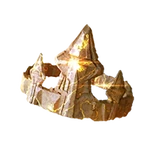
\includegraphics[width=1em,height=1em]{images/kingsrock.png} & Politoed \\
    Slowpoke & 50 Slowpoke candy + 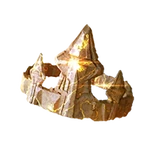
\includegraphics[width=1em,height=1em]{images/kingsrock.png} & Slowking \\
    Onix & 50 Onix candy + 
\includegraphics[width=1em,height=1em]{images/metalcoat.png} & Steelix \\
    Scyther & 50 Scyther candy + 
\includegraphics[width=1em,height=1em]{images/metalcoat.png} & Scizor \\
    Seadra & 100 Horsea candy + 
\includegraphics[width=1em,height=1em]{images/dragonscale.png} & Kingdra \\
    Porygon & 25 Porygon candy + 
\includegraphics[width=1em,height=1em]{images/upgrade.png} & Porygon2 \\
    Poygon2 & 100 Porygon candy + 
\includegraphics[width=1em,height=1em]{images/sinnohstone.png} & Porygon-Z \\
    Lickitung & 100 Lickitung candy + 
\includegraphics[width=1em,height=1em]{images/sinnohstone.png} & Lickilicky \\
    Tangela	& 100 Tangela candy + 
\includegraphics[width=1em,height=1em]{images/sinnohstone.png} & Tangrowth \\
    Electabuzz & 100 Elekid candy + 
\includegraphics[width=1em,height=1em]{images/sinnohstone.png} & Electivire	\\
    Magmar & 100 Magby candy + 
\includegraphics[width=1em,height=1em]{images/sinnohstone.png} & Magmortar	\\
    Sneasel & 100 Sneasel candy + 
\includegraphics[width=1em,height=1em]{images/sinnohstone.png} & Weavile	\\
    Togetic & 100 Togepi candy + 
\includegraphics[width=1em,height=1em]{images/sinnohstone.png} & Togekiss	\\
    Yanma & 100 Yanma candy + 
\includegraphics[width=1em,height=1em]{images/sinnohstone.png} & Yanmega	\\
    Gligar & 100 Gligar candy + 
\includegraphics[width=1em,height=1em]{images/sinnohstone.png} & Gliscor	\\
    Murkrow & 100 Murkrow candy + 
\includegraphics[width=1em,height=1em]{images/sinnohstone.png} & Honchkrow	\\
    Misdreavus & 100 Misdreavus candy + 
\includegraphics[width=1em,height=1em]{images/sinnohstone.png} & Mismagius	\\
    Piloswine & 100 Swinub candy + 
\includegraphics[width=1em,height=1em]{images/sinnohstone.png} & Mamoswine	\\
    Dusclops & 100 Duskull candy + 
\includegraphics[width=1em,height=1em]{images/sinnohstone.png} & Dusknoir	\\
    Aipom & 100 Aipom candy + 
\includegraphics[width=1em,height=1em]{images/sinnohstone.png} & Ambipom	\\
    Roselia & 100 Budew candy + 
\includegraphics[width=1em,height=1em]{images/sinnohstone.png} & Roserade	\\
    Applin & 200 Applin candy + 20 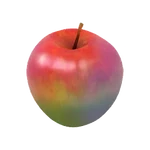
\includegraphics[width=1em,height=1em]{images/tartapple.png} & Flapple \\
    Applin & 200 Applin candy + 20 
\includegraphics[width=1em,height=1em]{images/sweetapple.png} & Appletun \\
    Zygarde 10\% & 50 
\includegraphics[width=1em,height=1em]{images/zygardecell.png} & Zygarde 50\% \\
    Zygarde 50\% & 200 
\includegraphics[width=1em,height=1em]{images/zygardecell.png} & Zygarde Complete \\
    Gimmighoul & 999 
\includegraphics[width=1em,height=1em]{images/gcoin.png} & Gholdengo \\
  \end{tabular}
  \caption{Evolutions dependent upon items\label{table:itemevolutions}}
\end{table}

\subsection{Eevolution}
\begin{figure}
\end{figure}
Evolution within the Eevee genus is a complicated and unique affair.
Eevee (the species) can evolve eight different ways.
Evolution can be driven by nicknames, deterministic across all eight targets,
  but this can be done only once per target per Trainer.
Otherwise, five targets require some condition, and are deterministic.
If none of the conditions are met, the evolution is nondeterministic,
  with three possible results.
For the nickname-based mechanic, give the Eevee you wish to evolve the nickname
  specified for the desired target from \autoref{table:eevee}.
When multiple deterministic evolutions are possible, all will be shown,
  and the Trainer can choose the target.
It is impossible to execute nondeterministic evolution when conditions for deterministic evolution are met.
When in doubt, check---if the evolution is deterministic, the ``Evolve'' button will show the target (or a silhouette thereof).
It will otherwise show a question mark.
Eevee's evolutions are strong Pokémon in the early game.
\begin{table}
\centering
\begin{tabular}{lrp{.5\textwidth}}
  Target & Nickname & Condition\\
  \Midrule
  Vaporeon & Rainer & Random\\
  Jolteon & Sparky & Random\\
  Flareon & Pyro & Random\\
  Sylveon & Kira & Earn 70 buddy hearts \\
  Espeon & Sakura & Walk 10 km with it as buddy,\newline evolve during the day\\
  Umbreon & Tamao & Walk 10 km with it as buddy,\newline evolve during the night\\
  Leafeon & Linnea & Evolve near an active 
\includegraphics[width=1em,height=1em]{images/rainylure.png} \\
  Glacion & Rea & Evolve near an active 
\includegraphics[width=1em,height=1em]{images/glaciallure.png} \\\\
\end{tabular}
  \caption{Eevolution\label{table:eevee}}
\end{table}

\section{Shadow and Purified Pokémon\label{sec:shadow}}
Team Rocket uses ``Shadow'' Pokémon modified for more attack
 and less defense capability than their base forms (for more details,
 see \autoref{sec:damage}).
Shadow Pokémon cost 20\% more Stardust than normal to teach second charged attacks or power up.
When captured from Team Rocket, they enter their own Shadow Pokédex.
Captured Shadow Pokémon always know the charged attack Frustration.
Only during certain special events can this charged attack be replaced,
 at which time a Charged TM is required as normal.
It's a pretty terrible Charged Attack, and this really degrades the
 Shadow Pokémon until it can be replaced.
A Shadow Pokémon can be taught a second Charged Attack at any time.
Frustration is preserved across evolution, as is Shadow status itself.
Shadow Pokémon cannot be traded.

Purification of a Shadow Pokémon has a cost in Stardust and Candy.
Purified Pokémon cost 10\% less than normal to evolve, teach second charged attacks, or power up.
Purification enters the Pokémon into its own Purified Pokédex,
 advances it to level 25 if not yet there,
 eliminates the attack bonus and defense penalty,
 replaces the primary charged attack with Return (exclusive to purified Pokémon),
 and increases each IV component by 2  (up to the usual max of 15).
Return is preserved across evolution, as is Purified status itself.
Purified Pokémon can be traded, but constitute a Special Trade (\autoref{sec:trades}).

It ought be obvious, but if you intend to purify a Shadow Pokémon, it
  is best to do so prior to any other development.
Shadow Pokémon are more expensive than normal to develop, while Purified Pokémon are cheaper.

\section{Regions, generations, myths, legends, and beasts\label{sec:regions}}
Each Pokémon is associated with one of eleven regions and one of nine generations.
Both can be determined by their Pokédex index (\autoref{table:regions}).
Whether Meltan and Melmetal (of the ``Unknown'' region) are Generation VII
  or Generation VIII is a raging and utterly inconsequential debate.
I place them in Generation VII because doing so saves a keystroke when using Roman numerals.
If you disagree, I encourage you to FAX your senator.
\begin{table}
\centering
\begin{tabular}{lcrr}
  Region & Generation & Start & End\\
  \Midrule
  Kanto & I & \#0001 & \#0151\\
  Johto & II & \#0152 & \#0251\\
  Hoenn & III & \#0252 & \#0386\\
  Sinnoh & IV & \#0387 & \#0493\\
  Unova & V & \#0494 & \#0649\\
  Kalos & VI & \#0650 & \#0721\\
  Alola & VII & \#0722 & \#0807\\
  Unknown & VII & \#0808 & \#0809\\
  Galar & VIII & \#0810 & \#0898\\
  Hisui & VIII & \#0899 & \#0905\\
  Paldea & IX & \#0906 & \#1025\\
\end{tabular}
\caption[Regions of the Pokémon world]{Regions of the Pokémon world (\textjapanese{ポケモンの世界})\label{table:regions}}
\end{table}
Legendary (\textjapanese{伝説のポケモン}) and Mythical (\textjapanese{幻のポケモン}) Pokémon
 are not generally seen in the wild.
They are members of the Pokémon mythos, heralds from times past and partly forgotten,
  some so rare that their existence is doubted.
Ultra Beasts (\textjapanese{ウルトラビースト}) literally assault our dimension from
  another via ``Ultra Wormholes''.
Such Pokémon never hatch from eggs (\autoref{sec:eggs}), and are not usually included in wild spawn groups (\autoref{sec:spawns}).
They are instead typically Research rewards, or captured in raids.
It is not usually possible to accumulate more than one or two examples of Mythical
  Pokémon\footnote{Marshadow, Celebi, Mew, Shaymin, Victini, Meloetta, Keldeo,
  Jirachi, Diancie, Zarude, Zygarde, and Volcanion.}, making them prime
  candidates for Bottle Caps.
They cannot be left in gyms (\autoref{sec:gyms}).
These Pokémon often comprise named sets (\autoref{table:namedmyths}).

\begin{table}
\begin{tabular}{lp{.65\textwidth}}
Group & Members\\
\Midrule
Legendary Birds & Articuno, Zapdos, Moltres\\
Galarian Birds & Galarian Articuno, Galarian Zapdos, Galarian Moltres\\
Legendary Beasts & Raikou, Entei, Suicune\\
Tower Duo & Lugia, Ho-Oh\\
Giants of Legend & Regigigas, Registeel, Regice, Regirock, Regieleki, Regidrago\\
Eon Duo & Latias, Latios\\
Weather Trio & Kyogre, Groudon, Rayquaza\\
Lake Guardians & Uxie, Mesprit, Azelf\\
Creation Trio & Dialga, Palkia, Giratina\\
Lunar Duo & Cresselia, Darkrai\\
Swords of Justice & Cobalion, Terrakion, Virizion, Keldeo\\
Forces of Nature & Tornadus, Thundurus, Landorus, Enamorus\\
Tao Trio & Reshiram, Zekrom, Kyurem\\
Aura Trio & Xerneas, Yveltal, Zygarde\\
Guardian Deities & Tapu Koko, Tapu Fini, Tapu Lele, Tapu Bulu\\
Light Trio & Solgaleo, Lunala, Necrozma\\
Hero Duo & Zacian, Zamazanta\\
Sea Guardians & Phione, Manaphy\\
Ultra Beasts & Nihilego, Buzzwole, Pheromosa, Xurkitree, Celesteela, Kartana, Guzzlord,
               Poipole, Naganadel, Stakataka, Blacephalon \\
\end{tabular}
\caption{Named collections of Legendary Pokémon\label{table:namedmyths}}
\end{table}

\begin{tipbox}[title=Kanto Starters]
The ``Kanto Starters'' refer to Bulbasaur, Charmander, and Squirtle, and sometimes
  also Pikachu and Eevee.
They are the initial partner Pokémon from various games.
\end{tipbox}

\section{Trends among species}
One thing to take away from \autoref{table:populations} is that the largest
  typings by population are the monotypes, representing 485 forms.
A majority of Pokédex have dual typing, but their diversity of typing means few dual types have much of a population.
Only Ground+Water, Flying+Normal, Bug+Poison, Grass+Ghost, Grass+Poison, Rock+Water, and Bug+Flying
  have more than ten members.
All monotypes have at least ten members except for Steel (9) and Flying (4).
\input{out/populations}
Scattering defense (max 400) against attack (max 420) for each type
  (including all species with that type in their typing) shows general
  balance.

\noindent{}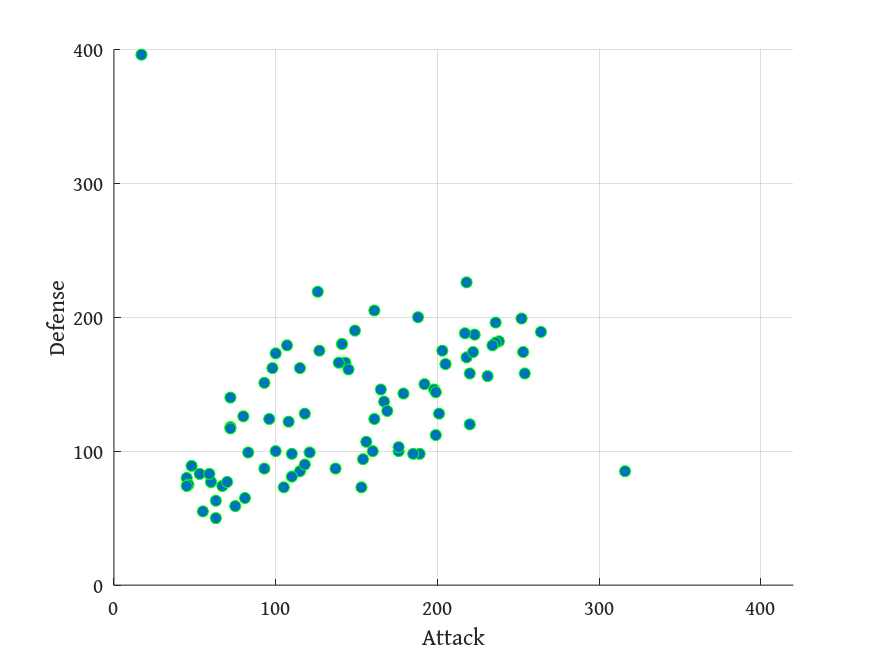
\includegraphics[width=.5\textwidth,keepaspectratio]{graph/BugDvA.png}
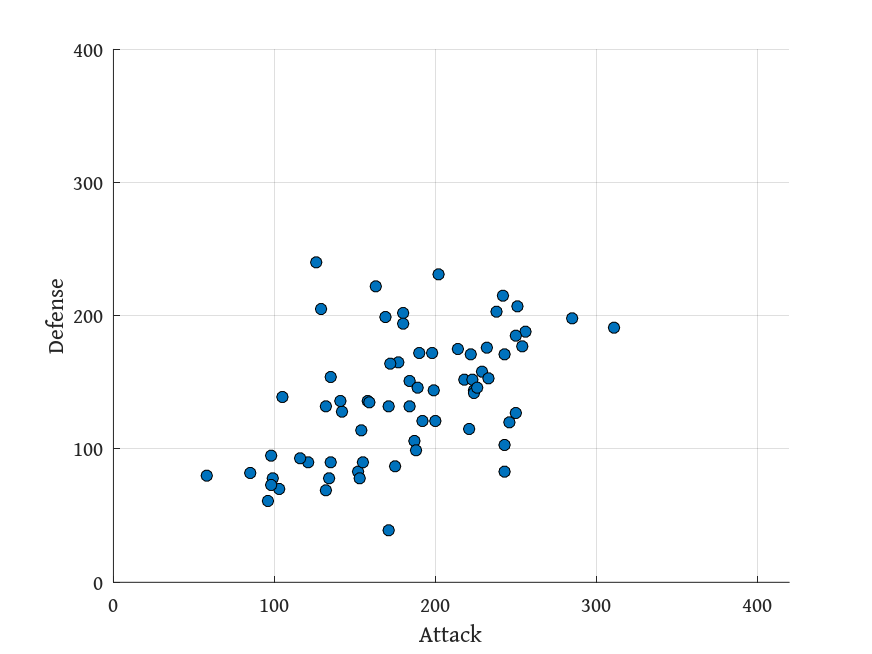
\includegraphics[width=.5\textwidth,keepaspectratio]{graph/DarkDvA.png}
\includegraphics[width=.5\textwidth,keepaspectratio]{graph/DragonDvA.png}
\includegraphics[width=.5\textwidth,keepaspectratio]{graph/ElectricDvA.png}
\includegraphics[width=.5\textwidth,keepaspectratio]{graph/FairyDvA.png}
\includegraphics[width=.5\textwidth,keepaspectratio]{graph/FightingDvA.png}
\includegraphics[width=.5\textwidth,keepaspectratio]{graph/FireDvA.png}
\includegraphics[width=.5\textwidth,keepaspectratio]{graph/FlyingDvA.png}
\includegraphics[width=.5\textwidth,keepaspectratio]{graph/GhostDvA.png}
\includegraphics[width=.5\textwidth,keepaspectratio]{graph/GrassDvA.png}
\includegraphics[width=.5\textwidth,keepaspectratio]{graph/GroundDvA.png}
\includegraphics[width=.5\textwidth,keepaspectratio]{graph/IceDvA.png}
\includegraphics[width=.5\textwidth,keepaspectratio]{graph/NormalDvA.png}
\includegraphics[width=.5\textwidth,keepaspectratio]{graph/PoisonDvA.png}
\includegraphics[width=.5\textwidth,keepaspectratio]{graph/PsychicDvA.png}
\includegraphics[width=.5\textwidth,keepaspectratio]{graph/RockDvA.png}
\includegraphics[width=.5\textwidth,keepaspectratio]{graph/SteelDvA.png}
\includegraphics[width=.5\textwidth,keepaspectratio]{graph/WaterDvA.png}
\begin{figure}[h]
\centering
\includegraphics[width=\textwidth,keepaspectratio]{graph/AllDvA.png}
  \caption{Defense vs Attack, all species\label{figure:alldva}}
\end{figure}

Now we scatter stamina (max 500) against attack (max 420):

\noindent{}\includegraphics[width=.5\textwidth,keepaspectratio]{graph/BugSvA.png}
\includegraphics[width=.5\textwidth,keepaspectratio]{graph/DarkSvA.png}
\includegraphics[width=.5\textwidth,keepaspectratio]{graph/DragonSvA.png}
\includegraphics[width=.5\textwidth,keepaspectratio]{graph/ElectricSvA.png}
\includegraphics[width=.5\textwidth,keepaspectratio]{graph/FairySvA.png}
\includegraphics[width=.5\textwidth,keepaspectratio]{graph/FightingSvA.png}
\includegraphics[width=.5\textwidth,keepaspectratio]{graph/FireSvA.png}
\includegraphics[width=.5\textwidth,keepaspectratio]{graph/FlyingSvA.png}
\includegraphics[width=.5\textwidth,keepaspectratio]{graph/GhostSvA.png}
\includegraphics[width=.5\textwidth,keepaspectratio]{graph/GrassSvA.png}
\includegraphics[width=.5\textwidth,keepaspectratio]{graph/GroundSvA.png}
\includegraphics[width=.5\textwidth,keepaspectratio]{graph/IceSvA.png}
\includegraphics[width=.5\textwidth,keepaspectratio]{graph/NormalSvA.png}
\includegraphics[width=.5\textwidth,keepaspectratio]{graph/PoisonSvA.png}
\includegraphics[width=.5\textwidth,keepaspectratio]{graph/PsychicSvA.png}
\includegraphics[width=.5\textwidth,keepaspectratio]{graph/RockSvA.png}
\includegraphics[width=.5\textwidth,keepaspectratio]{graph/SteelSvA.png}
\includegraphics[width=.5\textwidth,keepaspectratio]{graph/WaterSvA.png}

\begin{figure}[hb]
\centering
\includegraphics[width=\textwidth,keepaspectratio]{graph/AllSvA.png}
  \caption{Stamina vs Attack, all species\label{figure:alldva}}
\end{figure}

\section{Cost groups\label{sec:costgroups}}
Each species is in one of four cost groups.
Group membership determines the cost of teaching Pokémon a second charged move,
  upgrading Max Moves (\autoref{sec:dmaxgmax}),
  walk distance for Candy,
  and purification.
All Legendary and Mythical Pokémon are in group 4 (the most expensive group).
\begin{table}
\centering
\begin{tabular}{lrrrrrr}
  Group & 2nd move   & Max 1 & Max 2 & Max 3 & Km & Purify\\
\Midrule
      1 & 10k + 25   & 50    & 100   & 40 XL & 1  &       \\
  Shadow& 12k + 30   &       &       &       & 1  & 1k + 1\\
Purified& 8k + 8   &       &       &       & 1  &         \\
      2 & 50k + 50   & 60    & 110   & 45 XL & 3  &       \\
  Shadow& 60k + 60   &       &       &       & 3  & 3k + 3\\
  Purified& 48k + 48   &       &       &       & 3  &     \\
      3 & 75k + 75   & 70    & 120   & 50 XL & 5  &       \\
  Shadow& 90k + 90   &       &       &       & 5  & 5k + 5\\
  Purified & 60k + 60 &   &    &   & 5 &                  \\
      4 & 100k + 100 & 80    & 130   & 55 XL & 20 &       \\
  Shadow& 120k + 120 &       &       &       & 20 & 20k + 20\\
Purified& 80k + 80 &   &    &   & 20 & \\
\end{tabular}
  \caption{Costs for the four groups\label{table:costs}}
\end{table}

\section{Freak Pokémon\label{sec:freaks}}
A few Pokémon have unique behaviors or mechanics.

\subsection{Morpeko\label{subsec:morpeko}}
Morpeko changes its form between ``Full Belly Mode'' and ``Hangry Mode''
  each time it uses a charged attack.
Upon becoming active, Morpeko is in Full Belly Mode, and Aura Wheel is an Electric attack.
In Hangry Mode, Aura Wheel is a Dark attack.
Morpeko cannot defend gyms, assault gyms, or participate in raids.

\subsection{Smeargle\label{subsec:smeargle}}
Smeargle is not generally available in the wild\footnote{When captured in the wild, it knows Splash and Struggle.}.
Instead, it sometimes photobombs pictures taken of your Buddy Pokémon.
Smeargle will then spawn nearby, exclusive to the affected Trainer.
If caught, this Smeargle knows the same moves as whatever Pokémon was being photographed.
Smeargle will not appear more than once per day.
Smeargle cannot be taught a second charged attack.

\subsection{Ditto and Zorua\label{subsec:ditto}}
At any time, there is a set of Pokémon which might actually be Ditto,
  a Pokémon impersonator (impokénator?).
When captured, the Pokémon will be revealed as Ditto, and Ditto Candy will take
  the place of expected Candy.
Ditto status is shared across Trainers, i.e. it is a property of the spawn, not the encounter.
In battle, Ditto adopts the moves, typing, ATK, and DEF of its opponent, but not its MHP\@.
The result is almost universally garbage, and Ditto can't be used in 3x3 anyway\footnote{It is one of two species banned from PvP, the other being Shedinja.}.
The spiteful fox Zorua copies your Buddy Pokémon when it spawns; if you have no Buddy
  Pokémon, it spawns as itself.

\subsection{Zygarde\label{subsec:zygarde}}
Zygarde is received from research in its ``10\%'' form.
It can evolve to a ``50\%'' form, and a subsequent ``Complete'' form.
Zygarde Candy exists, but is not used for these evolutions.
Instead, ``Zygarde Cells'' are found on Routes, and can be stored in the Zygarde Cube
 (received at the same time as Zygarde 10\%).
The Cube can hold up to 300 cells, and cannot be removed from the bag.
Up to three cells can be collected per calendar day (more than three can spawn).
A route will not necessarily present a cell.
Cells are only generated the first time a route is taken each day, and more than one per route is very rare.
Cells usually show up near the end of a route, and disappear if the route is marked complete.

\subsection{Vivillon\label{subsec:vivillon}}
Remember postcards (\autoref{sec:capacities})?
Each Gift received from another Trainer bears a postcard, indicating the Gift's origin.
These postcards can be saved.
The globe is partitioned into eighteen regions (\autoref{figure:vivillonregions}),
  and a different Vivillon form is associated with each.
Upon pinning three, nine, or multiples of fifteen postcards from a region (but not more than thrice per calendar day),
  that region's Vivillon Collector medal (\autoref{sec:medals}) increases
  by a tier, and the Trainer encounters Scatterbug.
The Vivillon into which this Scatterbug evolves (via Spewpa) takes that region's form.
\begin{figure}
\centering
\includegraphics[keepaspectratio,width=\textwidth]{images/vivillonregions.png}
\caption{Munda est omnis divisia in partes duodeviginti\label{figure:vivillonregions}}
\end{figure}

\subsection{Furfrou, Spinda, and Unown\label{subsec:furfrou}}
Easily my most despised Pokémon, Furfrou has many forms.
Some are event-specific.
Some are region-specific.
All are worthless.
Should one for some reason wish to do so, a Trainer can change Furfrou's form
  at any time for 25 Furfrou Candy and 10,000 Stardust,
Furfrou at least has the decency to be easily caught, unlike the contemptible Unown.
Unown has 28 forms: one for each letter of the Latin alphabet, and two
  resembling deformed sperm.
In a grim future Trainers hunt new Unown, trading Shiny Octothorpes and
  Crowned Ampersands and Mega U+03CC GREEK SMALL LETTER OMICRON WITH TONOS.
Spinda has twenty visually distinct forms, but only nine have been released.
We wait with bated breath for the other eleven.

\subsection{Multiple type-distinct non-regional forms}
Each of these Pokémon has multiple forms with different attacks and types.
Wormadam's Plant, Sandy, and Trash forms evolve from three different Burmy,
 which differ only in appearance.
Cherrim's Sunshine form spawns only in sunlight; the Overcast form spawns otherwise.
Kyurem boasts Black and White forms capable of fusing with Reshiram.
Castform has four weather-specific forms.
The three alternative forms of Deoxys (Attack, Defense, and Speed) each take a stat to the extreme.
Palkia, Dialga, and Giratina each have an ``Origin'' form.
Shaymin's Sky form has the same attacks as its Land form, but adds Flying to its typing.

\subsection{Meltan\label{subsec:meltan}}
Meltan only appears when the Mystery Box is in use\footnote{Though a Meltan encounter ends the ``Let's GO, Meltan'' Special Research.}.
Charging the Mystery Box requires linking a Pokémon HOME account and transporting
  a Pokémon to it.
Meltan evolves into the interesting Melmetal, and the Mystery
  Box spawns pretty continuously for an hour should you need harvest some Stardust
  the hard way.

\subsection{Gimmighoul\label{sec:gimmighoul}}
Another one requiring interaction with the wider Pokémon empire, this time
 the Nintendo Switch games \textit{Pokémon Scarlet} or \textit{Pokémon Violet}.
Sending postcards to one of these games (whatever that means) earns you the Coin Bag,
 which functions as a Gimmighoul-specific incense for half an hour.
The Gimmighoul coins necessary to evolve into Gholdengo can be acquired by capturing
 Gimmighoul, or spinning Golden Pokéstops.
Pokéstops become golden with active Golden Lures.
Golden Lures are acquired by sending multiple postcards to these same games.

\begin{tipbox}[title=Galar First Partners]
The ``Galar First Partners'' refer to Grookey, Scorbunny, and Sobble, the
initial partner Pokémon from \textit{Sword and Shield}.
\end{tipbox}
